\documentclass{beamer}
\usetheme{Copenhagen}
\beamertemplatenavigationsymbolsempty

\usepackage{tikz}
\usetikzlibrary{arrows,shapes}
\definecolor{DarkBlue}{rgb}{0.1,0.1,0.5}
\usetikzlibrary{positioning}

%\setbeamercolor{frametitle}{fg=white}
%\setbeamercolor{background canvas}{bg=black}
%\setbeamercolor{normal text}{fg=white}

% Title page details:
\title{Genetic signatures of evolutionary rescue}
\author{Matthew Osmond}
\institute{Department of Ecology and Evolutionary Biology\\ University of Toronto}
\date{\today}

\begin{document}

% ==============================================

\begin{frame}
	\titlepage
\end{frame}

% ==============================================

% at least 27 yrs of theory on evol rescue: we know a lot about when and how rescue should occur
% a large and quickly growing number of experiments of increasing complexity and detail: verifying theory and discovering additional factors
% many examples of drug resistance, eg HIV, in asexual microbes: stressing an applied need to understand rescue for human health
% a big question that remains is: how common is rescue in wild sexual species? conservation angle
% evidence of the excitement around this question: a recent spike in claims for rescue in wild sexual species (amaranthus, killifish, arabidopsis, bats, etc)
% however, still unclear how confidently we can identify rescue from (predominately) contemporary genetic data
% this is a new direction for rescue theory

% ==============================================

\begin{frame}
	\frametitle{Evolutionary rescue}

	\begin{center}
	\begin{tikzpicture}
		\node (a) {\includegraphics[width=1\linewidth]{../images/er-trend.png}};\pause
		\fill[opacity=.75, color=white] (a.north west) rectangle (a.south east);
		\node[text width=\linewidth, yshift = 20]{
			\begin{itemize}
				\item we have a lot of theory on when/how rescue should happen \pause
				\item we have a lot of examples of rescue in asexual microbes \pause
				\begin{itemize}
					\item important for drug resistance \pause
				\end{itemize}
				\item a big question remains \pause
			\end{itemize}

			\begin{block}{Q}
				How common is rescue in wild sexual species? \pause
			\end{block}

			\begin{itemize}
				\item important for conservation
			\end{itemize}
		};
	\end{tikzpicture}
	\end{center}

\end{frame}

% ==============================================

% \begin{frame}
% 	\frametitle{Evolutionary rescue}
%
% 	\begin{itemize}
% 		\item we have a lot of theory on when/how rescue should happen \pause
% 		\item we have a lot of examples of rescue in asexual microbes \pause
% 		\begin{itemize}
% 			\item important for drug resistance \pause
% 		\end{itemize}
% 		\item a big question remains \pause
% 	\end{itemize}
%
% 	\begin{block}{Q}
% 		How common is rescue in sexual species? \pause
% 	\end{block}
%
% 	\begin{itemize}
% 		\item important for conservation
% 	\end{itemize}
%
% \end{frame}

% ==============================================

\begin{frame}
	\frametitle{How common is rescue in wild sexual species?}

	A lot of excitement around this question right now, eg \pause

	\begin{itemize}
		\item Hares rescued from lack of snow {\tiny Mills et al. 2018}
		\begin{center}
			\includegraphics[width=0.5\linewidth]{../images/hares.png} \pause
		\end{center}
		\item Bats rescued from white-nose syndrome {\tiny Gignoux-Wolfsohn et al. 2018} \pause
		\item Killifish rescued from pollution {\tiny Oziolor et al. 2019} \pause
		\item \textit{Amaranthus tuberculatus} rescued from herbicides {\tiny Kreiner et al. 2019} \pause
		\item \textit{Arabidopsis thaliana} rescued from dry new climate {\tiny Fulgione et al. 2022}
	\end{itemize}

\end{frame}

% ==============================================

\begin{frame}
	\frametitle{How common is rescue in wild sexual species?}

	\begin{itemize}
		\item for most wild species all we have is contemporary data \pause
	\end{itemize}

	\begin{block}{Q}
		Can we infer past rescue from a bunch of genomes?
	\end{block}

	\begin{center}
		\includegraphics[width=0.75\linewidth]{../images/code.jpg}
	\end{center}

\end{frame}

% ==============================================

% coalescent framework for detecting selection and demography
% work with Coop on signatures of rescue: difficult/impossible to differentiate sweep+bottleneck from any data, but especially summary statistics?

% ==============================================


\begin{frame}
	\frametitle{Can we infer past rescue from a bunch of genomes?}

	\begin{center}
	\begin{tikzpicture}[overlay, remember picture, axis/.style={very thick, ->, >=stealth', line join=miter}]

		\node[text width = \linewidth, yshift = 80] (list) {
			\begin{itemize}
				\item Graham Coop and I started down this path {\tiny Osmond \& Coop 2020} \pause
				\item coalescent model of rescue via a selective sweep\pause
			\end{itemize}
		};

		\begin{scope}[scale = 0.75, xshift = -90, yshift = -25]
			\only<3-7>{
				\draw[very thick] (-3,-2) -- (3,-2);
				\draw[very thick, ->, >=stealth'] (-3,-2) -- (-3,2);
				\node[rotate=90] at (-4,0) {absolute fitness};
				\draw[gray, dashed] (-3,0)  -- (3,0);
				\node[gray] at (2,-0.25) {replacement};
				\node[] at (-3.25,0) {1};
				\node[] at (-2,-2.25) {aa};
				\node[] at (0,-2.25) {Aa};
				\node[] at (2,-2.25) {AA};
				\node[] at (0,-3) {genotype};
			}
			\only<4-7>{
				\draw[fill=red, red] (-2,-0.5) circle (0.1);
				\node[red] at (-2,-1) {$1-d$};
			}
			\only<5-7>{
				\draw[fill=black] (0,0.45) circle (0.1);
				\node[] at (0,0.95) {$(1-d)(1+s/2)$};
			}
			\only<6-7>{
				\draw[fill=DarkBlue] (2,1.4) circle (0.1);
				\node[DarkBlue] at (2,1.9) {$(1-d)(1+s)$};
			}
		\end{scope}

		\begin{scope}[xshift=80, yshift=-25, scale = 0.4]
			\only<7>{
				\foreach \x in {-5,-4,...,5}{% Two indices running over each
					\foreach \y in {-5,-4,...,5}{% node on the grid we have drawn
						\node[draw,circle,inner sep=2pt,fill=red, red] at (\x,\y) {};
								% Places a dot at those points
					}
				}
				\node[draw,circle,inner sep=2pt,fill] at (5,-5) {};
				\node[] at (5,-5.75) {start with $1$ Aa};
			}
		\end{scope}

		\only<8-12>{
			\node[below = 0cm of list, xshift = -100] (dynamics) {
				\includegraphics[width=0.5\linewidth]{../images/rescueSGVhard_dynamics_talk_1.pdf}
			};
			\node[anchor=south east, yshift=10] at (dynamics.south east) {\tiny present};
			\node[anchor=south west, xshift=20, yshift=10] at (dynamics.south west) {\tiny past};
		}

		\visible<9-13>{
			\node[xshift = 100, yshift = 50, draw, rectangle, rounded corners, fill=black] (k) {
				\textcolor{white}{$k=2$}
			};
			\begin{scope}[xshift = 140, yshift = 0]
				\draw[line width=1] (-1,0.2) -- (1,0.2);
				\draw[line width=1] (-1,-0.2) -- (1,-0.2);
		 		\node[draw, star, star points=5, red, fill=red!20, star point ratio=0.5] at (0,0.2) {};
		 		\node[draw, star, star points=5, red, fill=red!20, star point ratio=0.5] at (0,-0.2) {};
				\draw[blue, very thick] (0.5,0.2-0.1) -- (0.5,0.2+0.1);
				\draw[blue, very thick] (0.5,-0.2-0.1) -- (0.5,-0.2+0.1);

				\def \xshift {-3}
				\def \yshift {-1}

				\draw[black,->,thick] (-1.25,0) -- (-2,0.5);
				\draw[black,->,thick] (-1.25,0) -- (-2,-0.5);

				\draw[line width=1] (-1+\xshift,0.2+\yshift) -- (1+\xshift,0.2+\yshift);
				\draw[line width=1] (-1+\xshift,-0.2+\yshift) -- (1+\xshift,-0.2+\yshift);
		 		\node[draw, star, star points=5, red, fill=red!20, star point ratio=0.5] at (0+\xshift,-0.2+\yshift) {};
				\draw[blue, very thick] (0.5+\xshift,0.2-0.1+\yshift) -- (0.5+\xshift,0.2+0.1+\yshift);
				\draw[blue, very thick] (0.5+\xshift,-0.2-0.1+\yshift) -- (0.5+\xshift,-0.2+0.1+\yshift);

				\draw[line width=1] (-1+\xshift,-0.2-\yshift) -- (1+\xshift,-0.2-\yshift);
		 		\node[draw, star, star points=5, red, fill=red!20, star point ratio=0.5] at (0+\xshift,-0.2-\yshift) {};
				\draw[blue, very thick] (0.5+\xshift,-0.2-0.1-\yshift) -- (0.5+\xshift,-0.2+0.1-\yshift);

				\node[rotate = 30] at (-1,0.75) {\tiny coalesce first};
				\node[rotate = -30] at (-1,-0.75) {\tiny recombine first};

			\end{scope}
		}
		\visible<10-13>{
			\node[xshift = 100, yshift = -75, text width = 0.4\linewidth, draw, rectangle, rounded corners, fill=blue!20] (math) {
				$p_{\mathrm{coal}}(k,t) = \binom{k}{2}\frac{1}{N(t)p(t)}$\\\vspace{0.5cm}
				$p_{\mathrm{rec}}(k,t) = k \frac{r}{2} [1-p(t)]$
			};
		}

		\only<11>{
			\node (timing) [below = -0.75cm of dynamics]{
				\includegraphics[width=0.5\linewidth]{../images/rescueSGVhard_timing_talk_1.pdf}
			};
		}
		\only<12>{
			\node (dynamics) [xshift = -100, below = 0cm of list]{
				\includegraphics[width=0.5\linewidth]{../images/rescueSGVhard_dynamics_talk_2.pdf}
			};
			\node (timing) [below = -0.75cm of dynamics]{
				\includegraphics[width=0.5\linewidth]{../images/rescueSGVhard_timing_talk_2.pdf}
			};
		}
		\only<13>{
			\node (dynamics) [below = 0cm of list, xshift=-100]{
				\includegraphics[width=0.5\linewidth]{../images/rescueSGVhard_dynamics_talk_2.pdf}
			};
			\node (timing) [below = -0.75cm of dynamics]{
				\includegraphics[width=0.5\linewidth]{../images/rescueSGVhard_timing_talk_3.pdf}
			};
		}
		\visible<14->{
			\node (stats) [xshift=-80, below = 0cm of list]{
				\includegraphics[width=0.5\linewidth]{../images/rescueSGVhard_heterozygosity_talk_3.pdf}
			};
		}
		\visible<15->{
			\node (stats2) [right=0cm of stats]{
				\includegraphics[width=0.5\linewidth]{../images/rescueSGVhard_tajimasD_talk.pdf}
			};
		}
		\visible<16->{
			\node[text width = \linewidth, below = 4cm of list] (conclusion) {
				\begin{itemize}
					\item conclusion: difficult to infer rescue from summary statistics
				\end{itemize}
			};
		}
	\visible<17->{
		\node[text width = \linewidth, below = 0cm of conclusion] {
			\begin{block}{Q}
				But what if we could observe the coalescent itself?
			\end{block}
		};
	}
	\end{tikzpicture}
	\end{center}

\end{frame}

% ==============================================

% what if we could see the coalecent trees themselves? does that give us more power to detect rescue? (Hejase et al 2022 say that summary statistics confound seln and demo)
% arabidopsis example (https://www.nature.com/articles/s41467-022-28800-z): used the trees, found bottleneck and sweeps but remains unclear how well their methodology can pick up rescue

% ==============================================

\begin{frame}
	\frametitle{But what if we could observe the coalescent itself?}

	\begin{itemize}
		\item recent advances allow us to infer the coalescent trees \pause
		\begin{itemize}
			\item ARGweaver {\tiny Rasmussen \& Siepel 2013} \pause
			\item Relate {\tiny Speidel et al. 2019} \pause
			\item tsinfer + tsdate {\tiny Kelleher et al. 2019, Wohns et al. 2022} \pause
		\end{itemize}
	\end{itemize}

	\begin{center}
		\includegraphics[width=\linewidth]{../images/ts.png}
	\end{center}

\end{frame}

% ==============================================

\begin{frame}
	\frametitle{But what if we could observe the coalescent itself?}

	\begin{itemize}
		\item with trees we can infer \textbf{recent} demography and evolution \pause
		\begin{itemize}
			\item Relate\\
			% \begin{center}
				\includegraphics[width=0.5\linewidth]{../images/relate_ne.png} \pause
			% \end{center}
			\item CLUES {\tiny Stern et al. 2019}\\
			% \begin{center}
				\includegraphics[width=0.75\linewidth]{../images/clues.png}
			% \end{center}
		\end{itemize}
	\end{itemize}

\end{frame}

% ==============================================

\begin{frame}
	\frametitle{But what if we could observe the coalescent itself?}

	\begin{itemize}
		\item in fact, trees already being used to infer rescue, eg \pause
		\begin{itemize}
			\item \textit{Amaranthus} herbicide resistance {\tiny Kreiner et al. 2022}
			% \begin{center}
				\includegraphics[width=0.75\linewidth]{../images/kreiner_plot.png} \pause
			% \end{center}
			\item \textit{Arabidopsis} colonizing Cape Verde {\tiny Fulgione et al. 2022}
			% \begin{center}
				\includegraphics[width=0.4\linewidth]{../images/fulgione_ne.png}
				\includegraphics[width=0.4\linewidth]{../images/fulgione_p.png}
			% \end{center}
		\end{itemize}
	\end{itemize}

\end{frame}

% ==============================================

% run simulations of rescue, infer trees, infer demography and selection -- can we detect rescue?

% ==============================================

\begin{frame}
	\frametitle{How well do inferred trees infer rescue?}

	\begin{block}{Q}
		How well do inferred trees infer rescue?\pause
	\end{block}

	\begin{itemize}
		\item simulate rescue via sweep with SLiM + msprime {\tiny Haller et al. 2019, Baumdicker et al. 2022} \pause
		\item infer trees from resulting variant data \pause
		\item infer demography and allele frequency dynamics from trees \pause
		\item compare with the truth
	\end{itemize}

\end{frame}

% ==============================================

\begin{frame}
	\frametitle{How well do inferred trees infer rescue?}

	\begin{itemize}
		\item control \#1: neutral Wright-Fisher \pause
		\begin{itemize}
			\item $L=10^7$, $U=2r=2.5\times10^{-8}$, $n=25$ \pause
		\end{itemize}
	\end{itemize}

	\begin{center}
		\includegraphics[width=\linewidth]{../images/wf_s0_trees.png}\\
		\pause
		\includegraphics[width=0.5\linewidth]{{../images/sim_10000K_-1d_0s_0.5h_2B_0u_1q_10000000L_1.25e-08r_0.75f_10n_25k_2.5e-08U_popsize}.png}
	\end{center}

\end{frame}

% ==============================================

\begin{frame}
	\frametitle{How well do inferred trees infer rescue?}

	\begin{itemize}
		\item control \#2: Wright-Fisher, s=0.01 \pause
		\begin{itemize}
			\item $L=10^7$, $U=2r=2.5\times10^{-8}$, $n=25$ \pause
		\end{itemize}
	\end{itemize}

	\begin{center}
		\includegraphics[width=\linewidth]{{../images/wf_s0.01_trees}.png}\\
		\pause
		\includegraphics[width=0.5\linewidth]{{../images/sim_10000K_-1d_0.01s_0.5h_2B_0u_1q_10000000L_1.25e-08r_0.75f_10n_25k_2.5e-08U_popsize}.png}
		\pause
		\includegraphics[width=0.5\linewidth]{{../images/sim_10000K_-1d_0.01s_0.5h_2B_0u_1q_10000000L_1.25e-08r_0.75f_10n_25k_2.5e-08U_freq_true-times}.png}
	\end{center}

\end{frame}

% ==============================================

\begin{frame}
	\frametitle{How well do inferred trees infer rescue?}

	\begin{itemize}
		\item control \#3: d=0, s=0.01 \pause
		\begin{itemize}
			\item $L=10^7$, $U=2r=2.5\times10^{-8}$, $n=25$ \pause
		\end{itemize}
	\end{itemize}

	\begin{center}
		\includegraphics[width=\linewidth]{{../images/d0_s0.01_trees}.png}\\
		\pause
		\includegraphics[width=0.5\linewidth]{{../images/sim_10000K_0d_0.01s_0.5h_2B_0u_1q_10000000L_1.25e-08r_0.75f_10n_25k_2.5e-08U_popsize}.png}
		\pause
		\includegraphics[width=0.5\linewidth]{{../images/sim_10000K_0d_0.01s_0.5h_2B_0u_1q_10000000L_1.25e-08r_0.75f_10n_25k_2.5e-08U_allelefreq}.png}
	\end{center}

\end{frame}

% % ==============================================
%
% \begin{frame}
% 	\frametitle{How well do inferred trees infer rescue?}
%
% 	\begin{itemize}
% 		\item rescue: d=0.005, s=0.01 \pause
% 		\begin{itemize}
% 			\item $L=10^7$, $U=2r=2.5\times10^{-8}$, $n=25$ \pause
% 		\end{itemize}
% 	\end{itemize}
%
% 	\begin{center}
% 		\includegraphics[width=\linewidth]{{../images/d0.005_s0.01_trees}.png}\\
% 		\pause
% 		\includegraphics[width=0.5\linewidth]{{../images/sim_10000K_0.005d_0.01s_0.5h_2B_0u_1q_10000000L_1.25e-08r_0.75f_10n_25k_2.5e-08U_popsize}.png}
% 		\pause
% 		\includegraphics[width=0.5\linewidth]{{../images/sim_10000K_0.005d_0.01s_0.5h_2B_0u_1q_10000000L_1.25e-08r_0.75f_10n_25k_2.5e-08U_allelefreq}.png}
% 	\end{center}
%
% \end{frame}

% ==============================================

\begin{frame}
	\frametitle{How well do inferred trees infer rescue?}

	\begin{itemize}
		\item rescue: d=0.005, s=0.02 \pause
		\begin{itemize}
			\item $L=10^7$, $U=2r=2.5\times10^{-8}$, $n=25$ \pause
		\end{itemize}
	\end{itemize}

	\begin{center}
		\includegraphics[width=\linewidth]{{../images/d0.005_s0.02_trees}.png}\\
		\pause
		\includegraphics[width=0.5\linewidth]{{../images/sim_10000K_0.005d_0.02s_0.5h_2B_0u_1q_10000000L_1.25e-08r_0.75f_10n_25k_2.5e-08U_popsize}.png}
		\pause
		\includegraphics[width=0.5\linewidth]{{../images/sim_10000K_0.005d_0.02s_0.5h_2B_0u_1q_10000000L_1.25e-08r_0.75f_10n_25k_2.5e-08U_allelefreq}.png}
	\end{center}

\end{frame}

% ==============================================

\begin{frame}
	\frametitle{Conclusion}

	\begin{itemize}
		\item trees contain a lot more information than summary statistics\pause
		\item can infer a coincident sweep and bottleneck in recent past
	\end{itemize}

	\begin{center}
		\includegraphics[width=0.75\linewidth]{{../images/sim_10000K_0.005d_0.02s_0.5h_2B_0u_1q_10000000L_1.25e-08r_0.75f_10n_25k_2.5e-08U_overlay}.png}
	\end{center}

\end{frame}

% ==============================================

% \begin{frame}
% 	\frametitle{Arabidopsis thaliana}
%
% 	\begin{alertblock}{To do}
% 		analyze trees, compare to pi
% 	\end{alertblock}
%
% \end{frame}

% ==============================================

\begin{frame}
	\frametitle{What is it that we can say?}

	\begin{alertblock}{causation}
		\begin{itemize}
			\item coincident sweep and bottleneck $\neq$ rescue \pause
		\end{itemize}
	\end{alertblock}

	\begin{alertblock}{rescue vs. adaptation}
		\begin{itemize}
			\item we have observed a population adapt and persist \pause
			\item how likely was extinction? \pause
			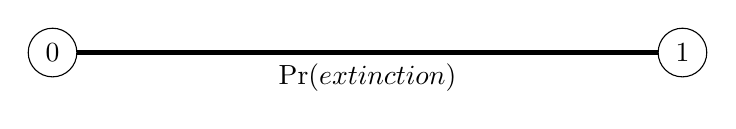
\begin{tikzpicture}
				\node[draw, circle] (0) at (0,0) {0};
				\node[draw, circle] (1) at (8,0) {1};
				\draw[ultra thick] (0) -- node[below] {$\Pr(extinction)$} (1) ;
			\end{tikzpicture}\pause
			\item $\Pr$(extinction)$=0 \implies$ adaptation \pause
			\item $\Pr$(extinction)$>0 \implies$ evolutionary rescue \pause
			\item larger $\Pr$(extinction)$ \implies$ more interesting rescue? \pause
			\item would be nice to estimate $\Pr$(extinction)
		\end{itemize}
	\end{alertblock}

		% rescue = survival with evolution (A) given extinction without (B)
		% \begin{equation}
		% \begin{aligned}
		% P(rescue) &= P(A|B) \\
		% &= P(A \cap B) / P(B) \\
		% &= [P(A) + P(B) - P(A \cup B)] / P(B) \\
		% &= [P(A) + 1 - P(B^c) - P(A \cup B)] / P(B) \\
		% &= [P(A) - P(B^c) + P(A^c \cap B^c)] / P(B)
		% \end{aligned}
		% \end{equation}



\end{frame}

% ==============================================

\begin{frame}
	\frametitle{Extensions}

	\begin{itemize}
		\item can extend to polygenic traits {\tiny Edge and Coop 2019, Stern et al 2021}
	\end{itemize}

\end{frame}

% ==============================================

\begin{frame}
	\frametitle{Thank-you}

	\begin{center}
		\includegraphics[width=1cm]{../images/nserc.png}

		\includegraphics[width=0.75\linewidth]{../images/leslie-lab.jpeg}


		\includegraphics[width=0.5cm]{../images/github.png} github.com/mmosmond/tsrescue
	\end{center}

\end{frame}

% ==============================================


% speidel et al 2019 show that they can infer demography better than SMC in recent time, 10^2 - 10^4 generations (fig 2)
% stern et al 2019 show that they can infer allele freq and selection very well, including recent strong selection (<10^2 gens, s<0.03) from SGV or DNM (fig 7a)
% stern et al 2019 used ARGweaver but later updated the software to work with Relate, which is what Fulgione used
% hejase et al 2022: relate and SIA better at detecting seln than sum stats when selection weak and DAF low (fig 2); CLUES tends to understimate strong seln coefficients with true trees (fig 3), CLUES very much underestimates s when using inferred Relate trees (fig 4) -- note that comparing this to stern et al 2019 means that the error is coming from Relate, and that ARGweaver should do better, compare fig 4 and s5 in hejase (clues better with argweaver, but still not great and a TON of variation)

\end{document}
